% Compile from this directory with: xelatex why_three_stage2.tex
\documentclass[11pt,a4paper]{article}
\usepackage{kotex}
\usepackage{amsmath,amssymb,booktabs,graphicx,geometry,hyperref}
\geometry{margin=25mm}
\graphicspath{{../results/}}
\hypersetup{colorlinks=true,urlcolor=blue}

\title{I01 후속 실험 2: ``세 활성 축'' 분기는 얼마나 안정적인가?}
\author{정확한 유한-$n$ 열분포와 단일 뒤집힘 동역학}
\date{2026년 10월 2일}

\begin{document}
\maketitle

\begin{abstract}
첫 I01 조건 지도에서 도입한 순열대칭 활성화 모형을 재검토한다.
세 활성 축의 바닥상태는 한 점의 미세조정이 아니라 유한 폭의
모수 구간에서 생긴다. 그러나 분기 개수의 엔트로피와 단일 축
전환을 허용하면 정지분포에서 세 축이 우세한 조건과 특정 분기가
관측시간 동안 고정되는 조건이 서로 다르다. 이것은 이전 노트의
``미세조정''이라는 표현을 정정하고 실제 장애물을 정량화한다.
\end{abstract}

\section{모형과 정확한 영온도 구간}
$n\ge4$개의 후보 축에 $s_i\in\{0,1\}$를 놓고
$m=\sum_i s_i$를 활성 축 수라 하자. $b>0$와 $r=-a/b$에 대해
\begin{equation}
\frac{V(m)}b=-r m+\frac{m(m-1)}2,\qquad
\frac{V(m+1)-V(m)}b=m-r.
\end{equation}
따라서 $2<r<3$이면 모든 $n\ge4$에서 유일한 바닥
\emph{활성 축 수}는 $m=3$이다. 이 구간의 폭은 1이다.
``세 축은 미세조정으로만 가능하다''는 이전 표현은 정확하지 않다.
더 정확한 문제는 $r$의 물리적 기원이 없고, 그 값이 왜
$(2,3)$에 들어가는지 설명하지 못한다는 것이다.
구간의 양 끝에서는 인접 활성 축 수와 축퇴한다.

축의 이름은 Hamiltonian에 없지만, $m=3$의 서로 다른 방향
분기는 $\binom n3$개다. 유한 $n$의 정확한 대칭상태가
저절로 한 방향 분기를 장시간 고정한다는 결론도 나오지 않는다.

\section{유한 선택온도: 엔트로피와 모수 창}
선택 역온도 $\beta_s$를 도입한 정확한 계수분포는
\begin{equation}
\Pr_{\beta_s}(m)=
\frac{\binom nm\exp[-\beta_sV(m)/b]}
{\sum_{j=0}^{n}\binom nj\exp[-\beta_sV(j)/b]}.
\end{equation}
여기서 $\beta_s$는 물리적 우주 온도를 측정한 값이 아니라
토이 확률분포의 매개변수다. $r=2.5$에서의 결과는 다음과 같다.
\begin{center}
\begin{tabular}{@{}ccccc@{}}
\toprule
$n$ & $\Pr_5(m=3)$ & $\Pr_{10}(m=3)$ &
$\beta_s$ for $\Pr(m=3)\ge0.9$ & $\beta_s$ for $\tau_{\rm exit}\ge100$\\
\midrule
4 & 0.874 & 0.988 & 5.51 & 11.98\\
6 & 0.890 & 0.990 & 5.21 & 12.79\\
20 & 0.734 & 0.971 & 7.37 & 15.20\\
50 & 0.506 & 0.926 & 9.33 & 17.03\\
\bottomrule
\end{tabular}
\end{center}
마지막 열의 수명 기준은 다음 절에서 정의한다. $n$이 커지면
다른 $m$과 방향 분기의 조합론적 수가 중요해진다.
예를 들어 $\beta_s=5$에서 $n=50$의 세 축 비율은 약 0.506이다.
정지분포가 $m=3$을 90\% 이상 갖는 $r$ 구간도 영온도 구간
$(2,3)$보다 좁다. $\beta_s=10$에서 그 폭은 $n=4$에서
약 0.658, $n=50$에서 약 0.534였다. 이 90\% 기준은
임의의 운영상 기준이지 자연상수는 아니다.

\section{단일 축 전환을 허용하면}
각 축이 단위율 Poisson 시계로 뒤집힘을 시도하고
Metropolis 규칙으로 수용된다고 가정한다.
$2<r<3$의 한 $m=3$ 분기에서 첫 탈출까지의 평균시간은
\begin{equation}
\tau_{\rm exit}=
\left[3e^{-\beta_s(r-2)}+(n-3)e^{-\beta_s(3-r)}\right]^{-1}.
\end{equation}
첫 항은 활성 축 하나가 꺼지는 사건, 둘째는 비활성 축
하나가 켜지는 사건이다. 중앙 $r=2.5$에서는
\begin{equation}
\tau_{\rm exit}=e^{\beta_s/2}/n.
\end{equation}
따라서 $\beta_s=10$에서 정지분포의 $m=3$ 확률은 높아도
첫 탈출 평균시간은 $n=4$에서 약 37.1, $n=50$에서 약 2.97
site-attempt 시간 단위뿐이다. $\tau_{\rm exit}\ge100$을
요구하면 $\beta_s\ge2\log(100n)$이 필요하다.

이것은 \emph{$m=3$ 집합에서 첫 이탈}의 시간이지 한 방향 분기가
영구적으로 바뀌는 시간은 아니다. 이탈 후 같은 분기로 돌아올
수도 있고 다른 분기로 갈 수도 있다. 그럼에도 첫 이탈이 잦다면
한 분기를 고정된 공간방향처럼 다루는 근거는 약해진다.
실제 우주의 긴 시간척도로 환산할 수 있는 모형도 아직 없다.

\begin{figure}[ht]
\centering
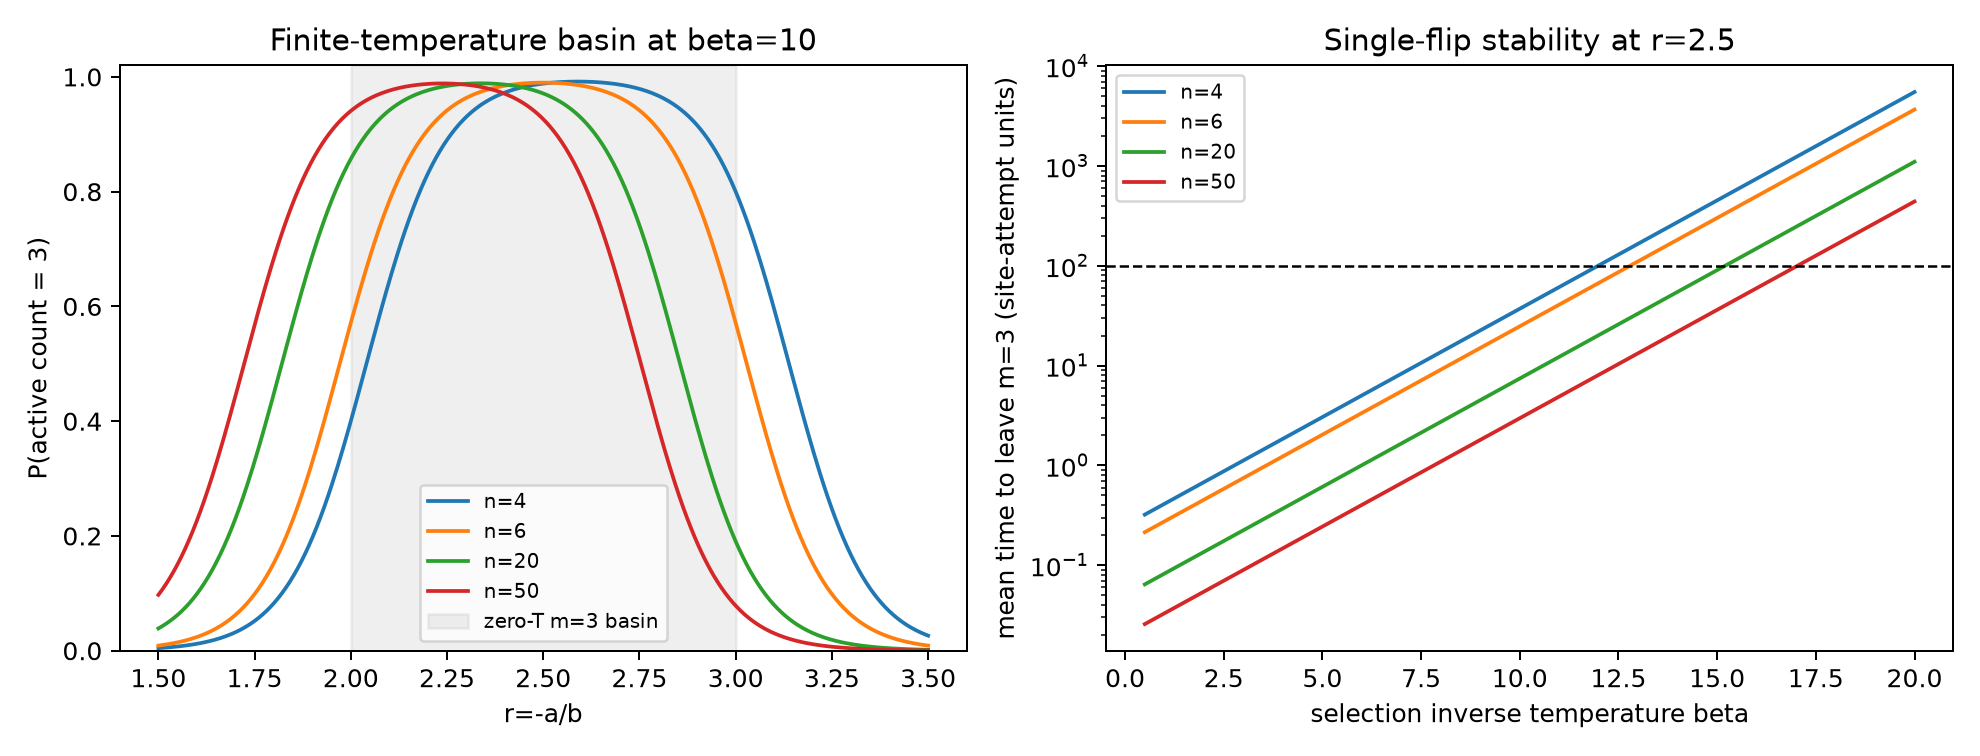
\includegraphics[width=\textwidth]{activation_stability.png}
\caption{왼쪽: 선택 역온도 10에서의 세 축 정지확률.
회색 영역은 영온도 $m=3$ 구간. 오른쪽: 중앙 모수에서
단일 뒤집힘 동역학의 첫 탈출시간.}
\end{figure}

\section{연구 판정과 재현성}
이 모형은 ``축을 사전 지목하지 않고 세 축 분기를 만들 수 없다''는
주장의 반례다. 그러나 세 축 \emph{개수}의 안정성과 한
\emph{방향} 분기의 고정은 다르다. $r$의 기원, 상호작용/전환 장벽,
물질 전파의 국소성, 세 활성 축의 계량적 기하가 모두 빠져 있다.
따라서 현재로서는 실제 공간의 선택 이론이 아니라 I01의
실패조건을 정량화하는 대조 모형이다.

코드는 \texttt{../src/relational\_atlas\_i01/geometry/activation\_stability.py}, 결과는
\texttt{../results/activation\_stability.json}, 회귀 검사는
\texttt{../tests/test\_activation\_stability.py}에 있다.
\end{document}
